\chapter{Related Work}

% NOTE: compares, contrasts, synthesizes, and provides introspection about the available knowledge for
% a given topic or field

\section{CERTIFY} % (fold)
\label{sec:CERTIFY}
This thesis is carried out in conjunction with the CERTIFY project \cite{certifyproject2023}.
% TODO: (aver) explain goals of CERTIFY

The National Institute for Standard and Technology has a few ongoing projects and white papers on security related
mitigation methods for IoT devices.
% section CERTIFY (end)


\section{DLT-based Asset-Tracking} % (fold)
\label{sec:DLT-based Asset-Tracking}
\cite{neisse2017blockchain} analyzed how blockchain-based approaches might be used for data accountability and
provenance tracking under the then recently released GDPR legislation, highlighting challenges of scalability and
considering sharding as a method to address it. \cite{neisse2017blockchain} Further they also mentioned issues of
clonability of the tracked assets, which we can also correlate to the physical assets that are tracked inside
blockchain.
% section DLT-based Asset-Tracking (end)


\section{Cybersecurity of IoT Devices} % (fold)
\label{sec:Cybersecurity of IoT Devices}

In order to maintain participation rights for only valid users/clients, Manufacturer Usage Descriptions, MUDs, are
getting more and more relevant, as also the National Institute for Standards and Technology, NIST, have been considering
their use cases. \cite{dodson2021securing}

\subsection{An Interledger Blockchain Platform for Cross-Border Management of Cybersecurity Information} % (fold)
\label{sub:An Interledger Blockchain Platform for Cross-Border Management of Cybersecurity Information}
A paper on management of cybersecurity information using blockchain and interledger technologies has already been
published back in 2020. \cite{skarmeta-interledger-management-2020} They identified two main challenges, the first being
a need to manage firmware and security patches and how it affected recertification.
They designed the framework in cooperation with the EU Cybersecurity Chain, worked as a main chain, while at lower
levels, national ledgers could be considered as side chains.
While periodically synchronizing with the main chain, there would be multiple side chains on the national level, one for
Information and Communication Technology, ICT, one as a Certification Chain and one as a Vulnerability chain.
Larger Information would be stored off-chain in a database.
% WARN: adjust later on
The composition of this framework agrees a lot with our design seen in Chapter~\ref{chap:Architecture and Design}.
Furthermore their use of the vulnerability chain to keep track of vulnerabilities, which can be announces and issued by
the manufacturers also is alike to our design.
% subsection An Interledger Blockchain Platform for Cross-Border Management of Cybersecurity Information (end)

\subsection{SRAM-based PUF Readouts} % (fold)
\label{sub:SRAM-based PUF Readouts}
For this thesis we will not be implementing a sophisticated Designated Accrediting Authority, DAA, leading to the
assumption, that it will be implemented as part of another thesis. For our use-case we will refer to simple
hardcoded authentication, with a key being provided for each device by us and trusted by us for simplicity.

Nonetheless the topic is still relevant from a cybersecurity perspective and there have been a few attempts at creating
secure keys out of SRAM readouts, such as \cite{vinagrero2023sram} or \cite{Niya_Jeffrey_Stiller_2020}.
We will also be considering using SRAM-based PUF readouts in our device configurations in order to get DIDs that are
absolutely unique for each device.
% subsection SRAM-based PUF Readouts (end)

\subsection{Device Fingerprinting} % (fold)
\label{sub:Device Fingerprinting}
For classification of device capabilities NIST has been considering the usage of MUDs, so that devices do not step out
the bounds of their official and appointed capabilities. \cite{dodson2021securing}
% subsection Device Fingerprinting (end)

% section Cybersecurity of IoT Devices (end)

\section{Decentralized Identity Management Technologies} % (fold)
\label{sec:Decentralized Identity Management Technologies}

In the quest for the right technologies, we are only considering open source projects, so that we may extend frameworks
and applications with modules to fit out needs, which why there may be many options not listed in here.

\begin{table}
	\caption{Comparison of Identity Management and Verified Credentials related Software}
	\label{tab:Comparison of Identity Management and Verified Credentials related Software}
	\begin{center}
		\begin{tabular}[c]{|p{3cm}|p{6.5cm}|p{5.5cm}|}
			\hline
			\textbf{Technology Name}                                                &
			Short Description                                                       &
			Main Features                                                             \\
			\hline
			Hyperledger Aries \cite{hyperledger:wiki}                               &
			creating, transmitting and storing verifiable digital credentials, (uses Indy per default,
			should be pluggable though)                                             &
			\begin{tableitemize}
				\item VC issuing
				\item Blockchain-agnostic
			\end{tableitemize}                                                  \\
			\hline
			Hyperledger Indy \cite{hyperledger:wiki}                                &
			Tools/Libraries for providing digital IDs rooted on Blockchains or DLTs &
			\begin{tableitemize}
				\item public read access
				\item Distributed Ledger for DID Management
			\end{tableitemize}                                \\
			\hline
			Hyperledger Fabric \cite{hyperledger:fabric:docs}                       &
			Framework to glue together blockchain, IdM and other DLT services to manage IoT devices, also
			supporting smart contracts; permissioned access                         &
			\begin{tableitemize}
				\item Distributed (Blockchain) OS
			\end{tableitemize}                                          \\
			\hline
			IoTeX \cite{iotex-bc-platform}                                          &
			Framework including blockchain to manage IoT devices                    &
			Does not fit our needs as it is permissionless                            \\
			\hline
			Sovrin                                                                  &
			\textbf{\textit{TODO}}                                                  &
			\textbf{\textit{TODO}}                                                    \\
			\hline
			IBM Platform                                                            &
			\textbf{\textit{TODO}}, works on top of Hyperledger Fabric              &
			\textbf{\textit{TODO}}                                                    \\
			\hline
		\end{tabular}
	\end{center}
\end{table}

\subsection{Decentralized Identity and Access Management for IoT (DIAM-IoT) Framework, 2020)} % (fold)
\label{sub:Decentralized Identity and Access Management for IoT}

\begin{figure}
	\begin{center}
		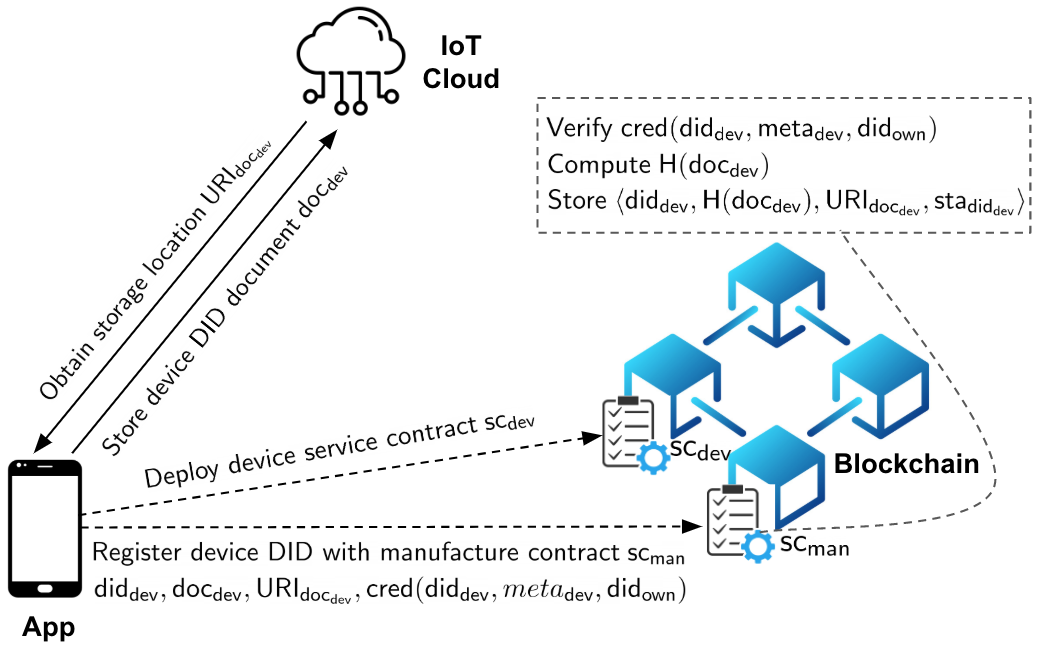
\includegraphics[width=0.95\textwidth]{figures/diam-iot-did-registration.png}
	\end{center}
	\caption{DIAM-IoT DID Registration Process \cite{diam-iot-2020}}
	\label{fig:diam-iot-did-registration}
\end{figure}

There has been a similar work in the field of our thesis, which has been made by \cite{diam-iot-2020}, who investigated
decentralized Identity and Access Management, IAM. They proposed a framework, DIAM-IoT, which incorporates DIDs and VCs
into the lifecycle of IoT devices, while building it up on blockchain as a bridge to connect IoT data silos.

They identified DID and global key-value databases as integral parts for building a self-sovereign identity system.

Their onboarding process includes the creation of a cryptocurrency wallet for manufacturers, through which each has to
stake some of the cryptocurrency tokens to deploy a smart contract for a new device. Those with poor products are
punished this way.

In contrast to our thesis, they refrained from using MUDs to specify device capabilities and designated each user with
their DID which is bound to a device that has a DID as well. Their use case is consumer oriented. Each user gets a
mobile application that can be used to do the device registration. A VC is generated by an IoT-Cloud after a successful
device binding (binding the user and a device). See Figure~\ref{fig:diam-iot-did-registration}.

The DIAM-IoT framework is blockchain agnostic, although they implemented it in the paper through the IoTeX Framework,
mentioned in Section~\ref{sec:IoTeX}. They mention scalability in their paper, there is no hard data presented.
The IoTeX documentation mentions scalability.
% subsection Decentralized Identity and Access Management for IoT (end)

\subsection{Hyperledger} % (fold)
\label{sub:Hyperledger}

The Hyperledger Foundation, run by the Linux Foundation, provides a great many technologies related to blockchains and
DLTs in general.

\subsubsection{Hyperledger Fabric} % (fold)
\label{sec:Hyperledger Fabric}
While there exist many blockchains, and with Ethereum having introduced smart contracts, enterprise use is growing. The
issue at hand, which Hyperledger Fabric tries to solve, is that these blockchains try to adapt to this environment,
which consists of identifiable participants, permissioned networks, high transaction throughput performance, therefore
also low latency of transaction confirmation and finally privacy and confidentiality of transactions and data relating
to business attractions. Hyperledger Fabric was designed solving these requirements in mind. \cite{hyperledger:fabric:docs}

It is also able to leverage consensus protocols, that do not necessitate cryptocurrency to incentivize mining or to
fuel smart contract execution. Due to its modularity it may be configured in any way users may require.

To address the issue of non-determinism mentioned in Section~\ref{sec:Smart Contract}, Hyperledger Fabric deploys a new
architecture \textit{execute-order-validate}, which enables the use of other languages. Execute a transaction and check
its correctness, thereby endorsing it, order transactions via a (pluggable) consensus protocol, and validate
transactions against an application-specific endorsement policy before committing them to the ledger. \cite{hyperledger:fabric:docs}
% subsubsection Hyperledger Fabric (end)

\subsubsection{Hyperledger Aries} % (fold)
\label{sec:Hyperledger Aries}
Hyperledger Aries is a graduated project from the Hyperledger foundation that focuses on on creating, transmitting and
storing verifiable digital credentials, with its infrastructure aimed at blockchain-rooted peer-2-peer interactions.

As mentioned in Section~\ref{sec:Verifiable Credentials and Identity Management}, Aries is already used to manage VCs
through compatible wallets in larger organizations such as the EU. Often used in conjunction with Indy and Ursa at
client layer...
% subsubsection Hyperledger Aries (end)

\subsubsection{Hyperledger Indy} % (fold)
\label{sec:Hyperledger Indy}
Hyperledger Indy is a blockchain platform designed for decentralized identity management.
It provides tools, libraries, and reusable components for creating and using independent digital identities rooted on blockchains or other distributed ledgers.
Indy focuses on providing a decentralized identity infrastructure that is secure, privacy-preserving, and interoperable.
It offers an implementation of the resolver and works closely with Hyperledger Aries to enable interoperability with other platforms.
Closely associated with the Sovrin Project
% subsubsection Hyperledger Indy (end)
% subsection Hyperledger (end)

\section{IoTeX} % (fold)
\label{sec:IoTeX}
IoTeX is a blockchain based framework focusing on decentralized application and IoT devices.
It provides functionalities such as blockchain, interconnections of decentralized applications, Dapps, using DIDs.
Architecturally is is quite similar to Ethereum, with a focus on IoT devices and also collaborating with Ethereum,
making it Ethereum Virtual Machine, EVM, compatible. Further DIDs are used to as on-chain identity framework that
enables users and devices to own their data, identity, and credentials. Further Real World Data Oracles convert real
world phenomena into verifiable and blockchain-ready data for use in the IoTeX Dapps.
IoTeX also supports Trusted Execution Environment, TEE, which is important for this thesis, i.e., for secure storage and
execution of certain applications and transactions.

Transactions are managed through the \textit{IOTX} token, e.g., to stake smart contracts as mentioned in
Section~\ref{sub:Decentralized Identity and Access Management for IoT}.

An advantage in using IoTeX would be, that it has already been used in IoT related projects, proving performance in the
area.

A shortcoming is, that the blockchain is not usable in a private environment, as it is permissionless and public.
Therefore in respect to this thesis, one needs to contrast, whether storing information is viable, which it does not for
us.

\begin{figure}
	\begin{center}
		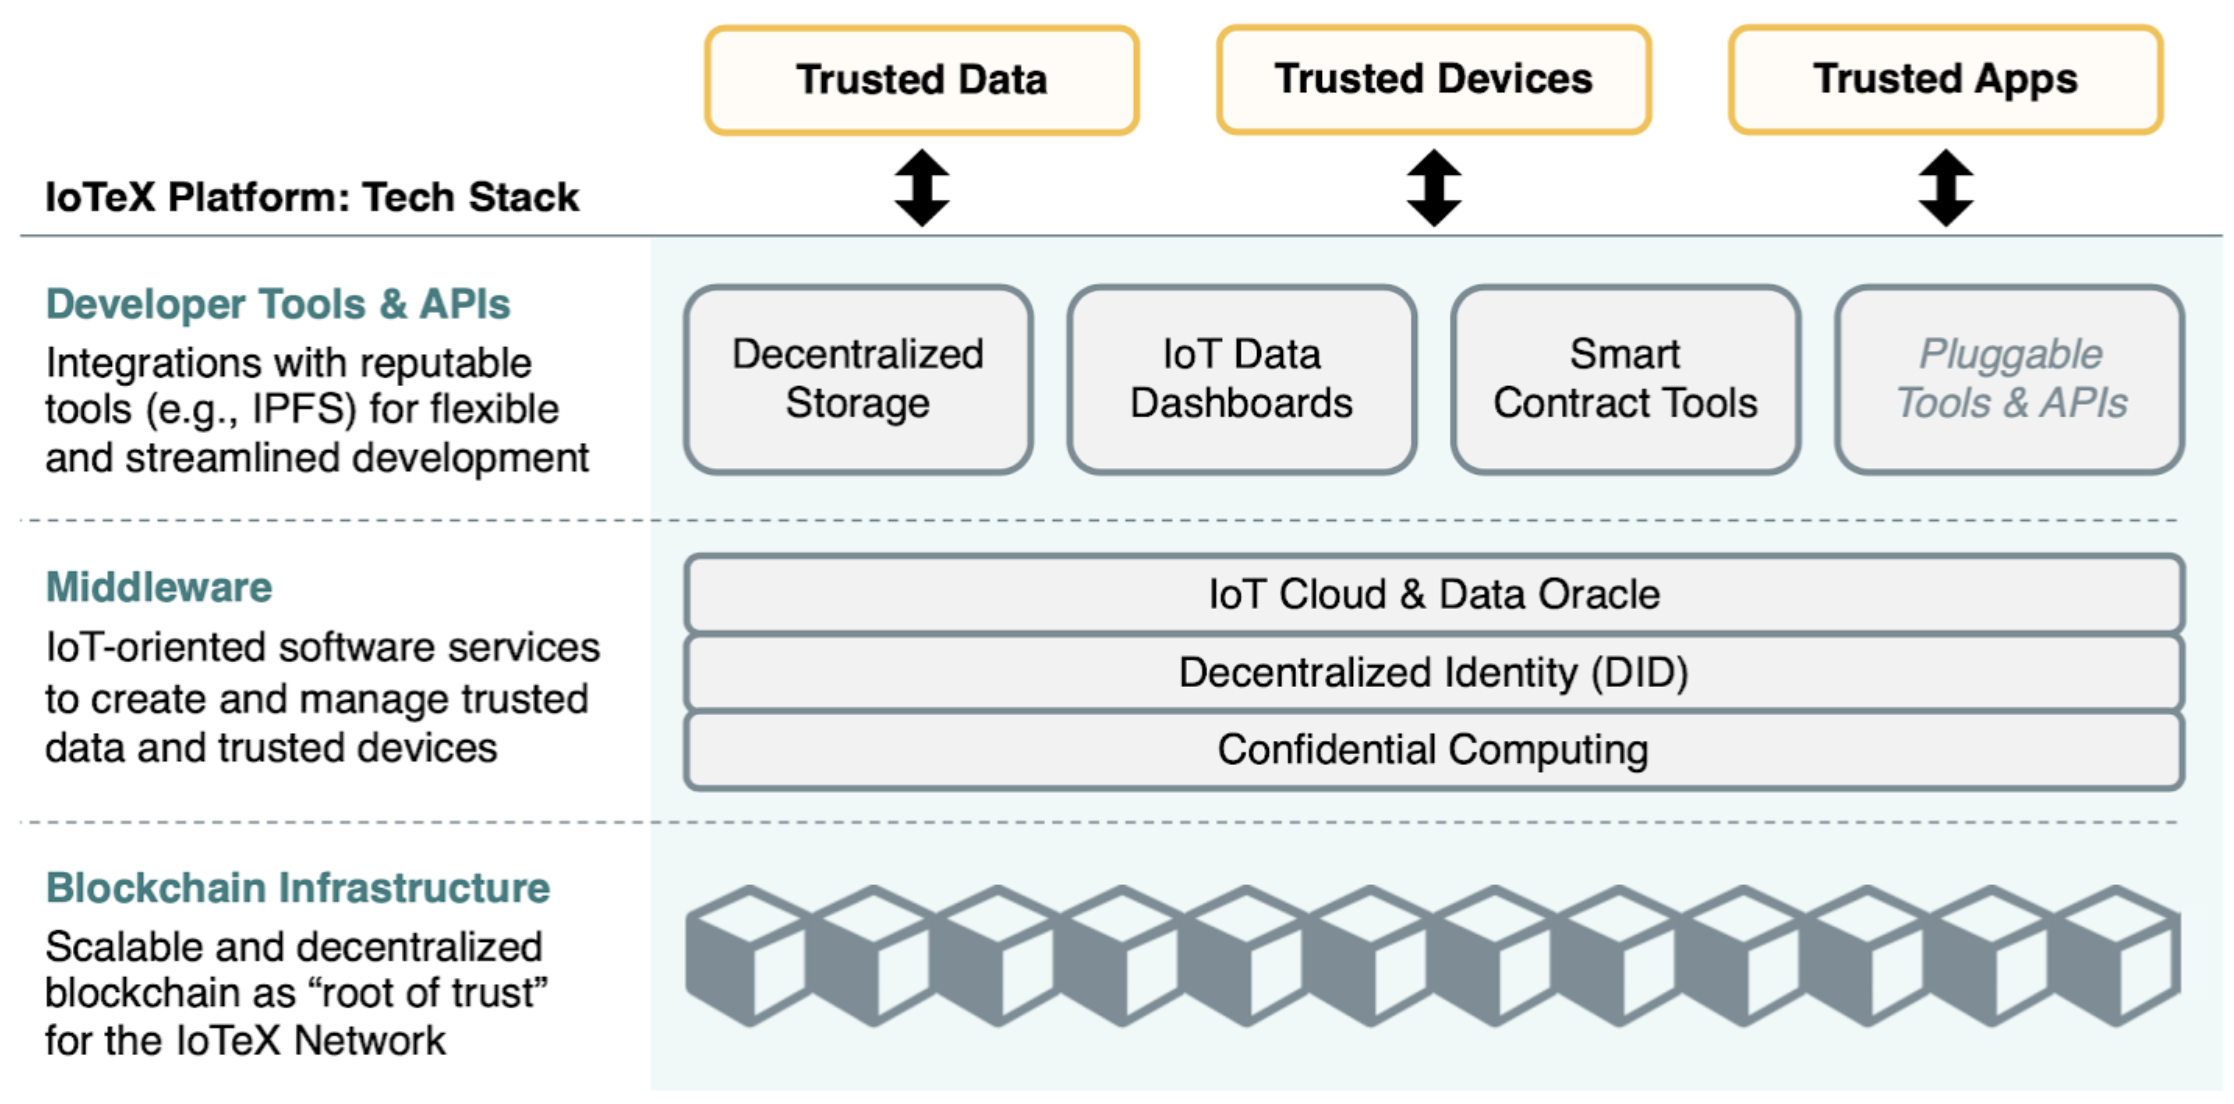
\includegraphics[width=0.95\textwidth]{figures/iotex-platform-stack.png}
	\end{center}
	\caption{IoTeX Platform Overview}
	\label{fig:iotex-platform-stack}
\end{figure}
% section IoTeX (end)

\section{Sovrin} % (fold)
\label{sec:Sovrin}
\textbf{\textit{TODO}}
% section Sovrin (end)

\section{Further non-DLT based IdM Frameworks} % (fold)
\label{sec:Further non-DLT based IdM Frameworks}
There are more frameworks to manage IoT devices, although they do not employ DLTs and therefore are not a focus of this
thesis.
% https://identity.foundation/
% https://www.dock.io/post/decentralized-identity
% https://www.devicehive.com/#open+source
% https://docs.devicehive.com/docs
% section Further non-DLT based IdM Frameworks (end)

% section Decentralized Identity Management Technologies (end)

\section{Blockchains} % (fold)
\label{sec:Blockchains}
\begin{table}
	\caption{Considered Blockchains}
	\label{tab:Considered Blockchains}
	\begin{center}
		\begin{tabular}[c]{|l|l|}
			\hline
			\textbf{Blockchain Name}                     & \textbf{Key Characteristics}                             \\
			\hline
			Hyperledger Iroha \cite{hyperledger:wiki}    & Permissioned Network                                     \\
			\hline
			Hyperledger Sawtooth \cite{hyperledger:wiki} & Permissioned Network, private, (aimed at enterprise use,
			scalable)                                                                                               \\
			\hline
			Ethereum                                     & Permissionless                                           \\
			\hline
			IoTeX \cite{iotex-bc-platform}               & Permissionless                                           \\
			\hline
			IBM Blockchain                               & \textbf{\textit{TODO}}                                   \\
			\hline
		\end{tabular}
	\end{center}
\end{table}

\subsection{Ethereum} % (fold)
\label{sub}

Ethereum is a widely known and used blockchain.

Also there is the Hyperledger Besu \cite{hyperledger:wiki} client to interact with Ethereum.

There is the Ethereum Virtual Machine...
% subsection Ethereum (end)

\subsection{Hyperledger Iroha} % (fold)
\label{sub:Hyperledger Iroha}

Hyperledger Iroha is a relatively new and unknown blockchain from the Hyperledger Foundation \cite{hyperledger:wiki}.
% subsection Hyperledger Iroha (end)

\subsection{IoTeX (Blockchain)} % (fold)
\label{sub:IoTeX-Blockchain}
See Section~\ref{sec:IoTeX}.
% subsection IoTeX (Blockchain) (end)

\subsection{IBM Blockchain} % (fold)
\label{sub:IBM-Blockchain}
We will not consider IBM Blockchain, as it is proprietary and builds up on Hyperledger products anyway.
% subsection IoTeX (Blockchain) (end)
% section Blockchains (end)

% NOTE: (aver) I if we wont be using RTOS, then we don't need a section on it
% \section{Real-Time Operating Systems} % (fold)
% \label{sec:Real-Time Operating Systems}
% \subsection{TockOS} % (fold)
% \label{sub:TockOS}
% The CERTIFY project considers using TockOS for their implementation on the IoT devices.
% Tock is a secure Real-Time Operating System, RTOS, designed to run on ARM and RISC-V based devices.
% % subsection TockOS (end)
% % section Real-Time Operating Systems (end)

\section{Tools} % (fold)
\label{sec:Tools}
\subsection{Docker} % (fold)
\label{sub:Docker}
Docker is a great alternative to Virtual Machines, VM, and makes it easier to distribute environment or images to end
users or developers.
% subsection Docker (end)
% section Tools (end)
